\documentclass{article}
\usepackage[a4paper, tmargin=1in, bmargin=1in]{geometry}
\usepackage[utf8]{inputenc}
\usepackage{graphicx}
\usepackage{parskip}
\usepackage{pdflscape}
\usepackage{listings}
\usepackage{hyperref}
\usepackage{caption}
\usepackage{subcaption}


\title{CS 754 : Advanced Image ProcessingAssignment 1}
\author{Meet Udeshi - 14D070007\\
  Arka Sadhu - 140070011\\
}
\date{\today}

\begin{document}
\maketitle

\section*{Q1}
\subsection*{A1.1}

Parameters chosen:
$$lambda = 0.5$$
$$alpha = max(eig(A'*A))$$

To compensate for the different intensity of the input and output image we have added the difference of the DC coefficients of the input
and output image and added it to the output image.

\begin{figure}[h!]
  % \centering
  \begin{subfigure}[t]{0.32\textwidth}
    \centering
    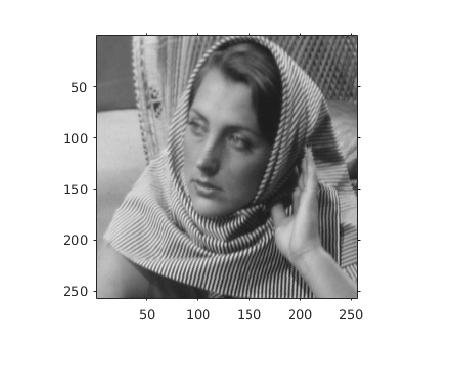
\includegraphics[scale=0.5]{images/original_image_barbara}
    \caption{Original Image Barbara}
    \label{Fig :1a}
  \end{subfigure}
  ~
  \begin{subfigure}[t]{0.32\textwidth}
    \centering
    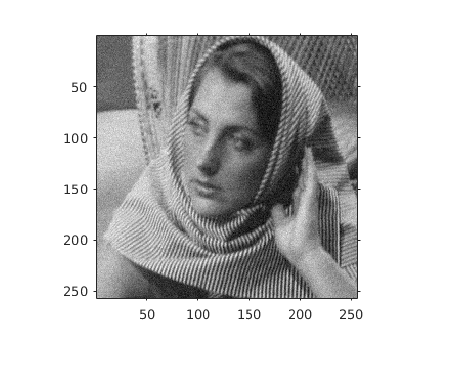
\includegraphics[scale=0.5]{images/noisy_image_barbara}
    \caption{Noisy Image Barbara}
    \label{Fig :1b}
  \end{subfigure}
  ~
  \begin{subfigure}[t]{0.32\textwidth}
    \centering
    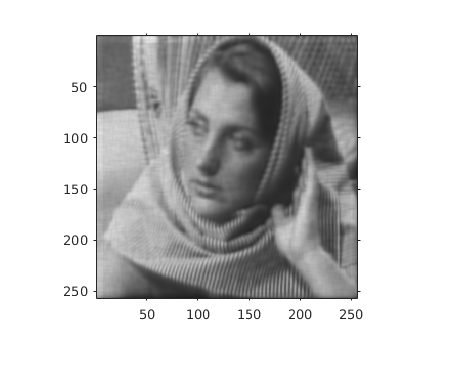
\includegraphics[scale=0.5]{images/denoised_image_barbara}
    \caption{Denoised Image Barbara}
    \label{Fig: 1c}
  \end{subfigure}

  \caption{Figures for Q1}
\end{figure}

\subsection*{A1.2}

\begin{figure}[h!]
  % \centering
  \begin{subfigure}[t]{0.5\textwidth}
    \centering
    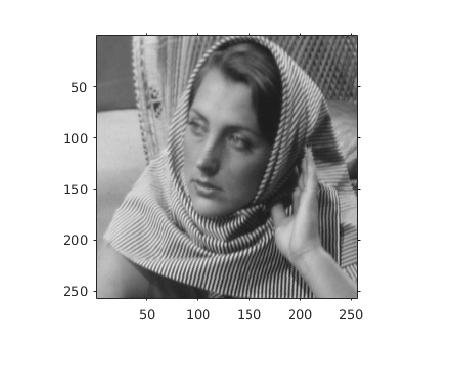
\includegraphics[scale=0.5]{images/original_image_barbara}
    \caption{Original Image Barbara}
    \label{Fig :1a}
  \end{subfigure}
  % ~
  \begin{subfigure}[t]{0.5\textwidth}
    \centering
    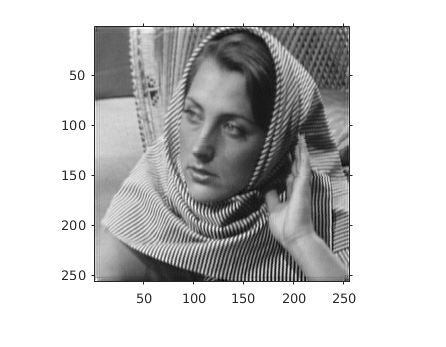
\includegraphics[scale=0.5]{images/phi_reconstructed_barbara}
    \caption{Reconstructed Image Barbara}
    \label{Fig :1b}
  \end{subfigure}
  \caption{Figures for Q2}
\end{figure}



\section*{Q3}
\subsection*{A3.1}
Assuming the image is of size NxN, and there are M filters. From equation (6) we note that, there are 4 terms to be considered.
The first term is : $\rho(f_{ik}.I_1)$.
To convert it into the form of $\rho(A_{j\rightarrow}v - b_j)$ where v = vectorized image $I_1$,
we need to construct $A_j$ such that its rows denote the derivative filter,
which on multiplication with v, will result in the derivative image.
Every possible $f_{i,k}$ is represented by one row of $A_j$,
such that $A_j\cdot v$ will give a column vector containing every term of the summation.
We will have to redefine $\rho_j(\vec{x})$ as $\sum_k \rho(x_k)$.


For all other terms $A_j$ will be constructed in the same way.
Only for the third and fourth term, we will take $f_{i,k}$ for only $i\in S_1/S_2$.
$b_j$ will be calculated as $f_{i,k}\cdot I$ for second and third term. Effectively $b_j = A_j\cdot I$.
For first and fourth term $b_j$ will be $0$.

Size of $A_j$ for first and second term is $N^2M\times N^2$, and for third and fourth term it will be $S_{(1|2)}M\times N^2$.

\subsection*{A3.2}
In equation (6) the first two terms are obtained from prior, while the last two terms are obtained from likelihood.\\
That is, the prior terms are:
$$\sum_{i,k} \rho (f_{i,k}\cdot I_1)$$
$$\sum_{i,k} \rho(f_{i,k} \cdot I_1 - f_{i,k} \cdot I)$$
The likelihood terms are :
$$\lambda \sum_{i \in S_1,k} \rho(f_{i,k}\cdot I - f_{i,k}\cdot I_1)$$
$$\lambda \sum_{i \in S_2,k} \rho(f_{i,k}\cdot I_1)$$

The prior used in this paper is the mixed Laplacian model, given by:
$$Pr(I) \approx \prod_{i,k}Pr(f_{i,k} \cdot I)$$
Approx sign is used, since we are assuming independence of derivative filters over space which is strictly not true.

The likelihood used in this paper is that the gradient of $I_1$ at all locations $S_1$ agree with the gradients of the input image $I$
and similarly gradient of $I_2$ at all locations $S_2$ agree with the gradients of the input image $I$. That is,\\
At all points $S_1$:
$$\nabla I_1 = \nabla I$$
At all points $S_2$
$$\nabla I_2 = \nabla I$$

\subsection*{A3.3}
Consider the third term :
$$\lambda \sum_{i \in S_1,k} \rho(f_{i,k}\cdot I - f_{i,k}\cdot I_1)$$
This can be reduced to
$$\lambda \sum_{i \in S_1,k} \rho(f_{i,k}\cdot I_2)$$
We have implicitly assumed that at points $S_1$ the gradient of $I_2$ is approximately zero (since the user will predominantly pick edges of $I_1$ and they are highly unlikely to coincide with the edges of $I_2$). Hence we expect this term to be even more sparse than the second term, which is $$\sum_{i,k} \rho(f_{i,k} \cdot I_2)$$
Since we have seen Gaussian model doesn't even fit $$\sum_{i,k} \rho(f_{i,k} \cdot I_2)$$ It is definitely not expected to fit the sparser term (which is the third term). In fact we can use a sparser model (instead of current mixed Laplacian) but we definitely cannot use Gauusian likelihood.

Similar argument can be provided for the fourth term. 

\end{document}

